\documentclass{article}
\usepackage[a4paper,top=2.5cm,bottom=2.5cm,left=2.5cm,right=2.5cm]{geometry}
\usepackage{makeidx}
\usepackage{natbib}
\usepackage{graphicx}
\usepackage{multicol}
\usepackage{float}
\usepackage{listings}
\usepackage{color}
\usepackage{ifthen}
\usepackage[table]{xcolor}
\usepackage{textcomp}
\usepackage{alltt}
\usepackage{ifpdf}
\ifpdf
\usepackage[pdftex,
            pagebackref=true,
            colorlinks=true,
            linkcolor=blue,
            unicode
           ]{hyperref}
\else
\usepackage[ps2pdf,
            pagebackref=true,
            colorlinks=true,
            linkcolor=blue,
            unicode
           ]{hyperref}
\usepackage{pspicture}
\fi
\usepackage[utf8]{inputenc}
\usepackage{polski}
\usepackage[T1]{fontenc}

\usepackage{mathptmx}
\usepackage[scaled=.90]{helvet}
\usepackage{courier}
\usepackage{sectsty}
\usepackage{amssymb}
\usepackage[titles]{tocloft}
\usepackage{doxygen}
\lstset{language=C++,inputencoding=utf8,basicstyle=\footnotesize,breaklines=true,breakatwhitespace=true,tabsize=8,numbers=left }
\makeindex
\setcounter{tocdepth}{3}
\renewcommand{\footrulewidth}{0.4pt}
\renewcommand{\familydefault}{\sfdefault}
\hfuzz=15pt
\setlength{\emergencystretch}{15pt}
\hbadness=750
\tolerance=750
\begin{document}
\hypersetup{pageanchor=false,citecolor=blue}
\begin{titlepage}
\vspace*{7cm}
\begin{center}
{\Large Life -\/-\/ Fight! \\[1ex]\large 0.\-1 }\\
\vspace*{1cm}
{\large Wygenerowano przez Doxygen 1.8.1.2}\\
\vspace*{0.5cm}
{\small Cz, 23 maj 2013 12:00:03}\\
\end{center}
\end{titlepage}
\pagenumbering{roman}
\tableofcontents
\pagenumbering{arabic}
\hypersetup{pageanchor=true,citecolor=blue}
\section{e\-Life}
\label{md_func}
\hypertarget{md_func}{}
Let's play game for life!

\subsection*{Strategia\-:}

x Co może być tu abstrakcyjnego? \begin{DoxyVerb}    x abstrakcja strategii, która będzie służyła obiektom do przetrwania
    x abstrakcja obiektu-zwierzaka, z jego podstawowymi cechami i funkcjami
    x abstrakcja planszy, którą łatwo można przeprogramować na inne systemy i biblioteki
\end{DoxyVerb}


x Propozycje funkcji życiowych\-: \begin{DoxyVerb}    x podstawowe potrzeby życiowe wg. Maslowa, piramida potrzeb    
    x sex, potrzeba utrzymania gatunku
    x jedzenie
    x picie
    x spanie
\end{DoxyVerb}


x Jak działają funkcje życiowe \begin{DoxyVerb}    x gdy niski poziom wody w obiekcie
            x uruchamiamy szukajWodę()?
                    x potem rozpaczliwieSzukajWodę()?
\end{DoxyVerb}


x Jak świat wpływa na obiekty? \begin{DoxyVerb}    x różne środowisko = różne wychowanie
    x odległość od wody = mniejsza szansa na przetrwanie?
\end{DoxyVerb}


x Rodzaje środowisk \begin{DoxyVerb}    x mapa różnych środowisk
    x pustynia
    x dżungla
    x knieje
    x góry
    x step
    x mazury
    x coś tam innego
\end{DoxyVerb}


x Jak pogrupować obiekty? \begin{DoxyVerb}    x roślinożercy i mięsożercy
    x ułożyć specjalną hierarchię członków gatunku
    x lista klanów? 
            x na jej czele głowy klanów
            x najstarsi, członkowie klanu
            x poniżej członkowie rodu niżsi i w jakichś sposób pogrupowani
\end{DoxyVerb}


x Mutacje? \begin{DoxyVerb}    x blisko spokrewnione klany mogą generować zmodyfikowane dziecka
    x kopulacja dwóch różnych gatunków powoduje stworzenie muła?
\end{DoxyVerb}


\subsection*{Klasy}

\subsubsection*{Związane z obsługą interfejsu na różnych systemach}


\begin{DoxyItemize}
\item {\ttfamily Okno}
\item {\ttfamily Wzorzec}
\begin{DoxyItemize}
\item Most?
\end{DoxyItemize}
\end{DoxyItemize}

\subsubsection*{Związane z tworzeniem mapy}


\begin{DoxyItemize}
\item {\ttfamily Mapa}
\begin{DoxyItemize}
\item 
\end{DoxyItemize}
\item {\ttfamily Wzorzec}
\begin{DoxyItemize}
\item Budowniczy?
\end{DoxyItemize}
\end{DoxyItemize}

\subsubsection*{Związane z tworzeniem obiektów na mapie}


\begin{DoxyItemize}
\item {\ttfamily Zwierzak}
\begin{DoxyItemize}
\item klasa abstrakcyjna, interfejs
\end{DoxyItemize}
\item {\ttfamily Zwierzak\-Roslinozerca \-: Zwierzak}
\begin{DoxyItemize}
\item na jej podstawie tworzone będą nowe klony roślinożernych zwierzątek
\end{DoxyItemize}
\item {\ttfamily Wzorzec\-:}
\begin{DoxyItemize}
\item Prototyp
\begin{DoxyItemize}
\item Służy do tworzenia nowych obiektów w czasie rzeczywistym 
\end{DoxyItemize}
\end{DoxyItemize}
\end{DoxyItemize}
\section{D\-N\-A\-: linie papilarne}
\label{md_GENETYKA}
\hypertarget{md_GENETYKA}{}
Witam w pierwszym wpisie z serii \char`\"{}\-D\-N\-A\char`\"{}. Poświęcę go liniom papilarnym. Pierwsze pytanie to czym one są. Dobra, widzimy jakieś wzorki, jednak nie jest to specjalnie dobre wyjaśnienie. Inna nazwa lini papilarnych to linie brodawkowe. Ta nazwa mówi już coś więcej. Jeszcze dokładniej można o nich powiedzieć, że są to wytwory skóry właściwej, bruzdy do których wnikają zakończenia nerwów. Mają je tylko ssaki naczelne i misie Koala.

Jak zapewne wiecie, dla każdego z nas są one niepowtarzalne. Nie ma możliwości by były dwie osoby z identycznym układem linii. Oczywiście taką właściwość człowiek wykorzystał. Zauważył ją w X\-I\-X wieku, jednak dopiero w latach 30. X\-X wieku zaczął ją wykorzystywać. Obecnie odciski palców są powszechnie używane przez policję i inne organizacje dbające o bezpieczeństwo. Dzięki nim (nierozważni) przestępcy mogą zacząć oglądać niebo w kratkę. Do zidentyfikowania sprawcy używa się tzw. minucji -\/ charakterystycznych cech jak np. rozwidleń, zagięć, haczyków itp. By mieć praktycznie 100\% pewność wystarczy już 12 identycznych minucji, jednak może wystarczyć mniej -\/ zależy to od ich rzadkości. Tyle też wystarczy by uznać odcisk za wiarygodny w świetle polskiego prawa. Aha. Nauka zajmująca się tymi sprawami to daktyloskopia.

Czasami można usłyszeć o zasadzie 3\-N Francisa Galtona. Mówi ona że linie są niepowtarzalne, niezmienne i nieusuwalne. O ile do pierwszych dwóch stwierdzeń nie można się przyczepić, to \char`\"{}nieusuwalne\char`\"{} nie jest już dobrym określeniem. W dzisiejszych czasach jeżeli tylko chcesz możesz się ich pozbyć. Oczywiście wiąże się to z zabiegiem dermatologicznym. Niestety zdarzają się sytuacje w których to natura podejmuje za nas decyzje. Dwie, bardzo rzadkie, choroby genetyczne wywołują brak linii papilarnych. Jest to spowodowane uszkodzeniem białka keratyna 14.

Na początku napisałem że wszyscy mają różne linie. Tutaj chciałbym wspomnieć, że nawet bliźnięta nie są wyjątkami. Mimo że mają takie samo D\-N\-A, ich linie papilarne są różne. Jednak o kwasie dezoksyrybonukleinowym napiszę za niedługo.

To tyle jeśli chodzi o linie papilarne. Zapraszam do następnego wpisu z serii \char`\"{}\-D\-N\-A\char`\"{}. Napiszę w nim o cechach dziedzicznych u człowieka -\/ już niebawem.

\subsection*{D\-N\-A\-: cechy dziedziczne}

Witam w drugim wpisie z serii \char`\"{}\-D\-N\-A\char`\"{}. Dziś napiszę o cechach dziedzicznych u człowieka. Jeżeli ktoś uważnie ogląda Dr. House'a, to w jednym odcinku chłopak stwierdził, że wie iż jest adoptowany już od 5 klasy -\/ znalazł w internecie informację, że podbródek który on ma, jest cechą dziedziczną, a żaden z jego przybranych rodziców go nie miał. Oczywiście nie chodzi mi tu abyśmy wszyscy zaczęli porównywać swoje cechy wyglądu z rodzicami. Powiedzmy że to co tutaj napiszę jest swoistą ciekawostką. Na dodatek niektóre cechy można odziedziczyć po przodkach (babci, dziadku, prababci).

Przejdźmy do konkretów. Dziedziczymy cechy fizyczne i psychiczne oraz biohemiczne. W psychicznych zawierają się m.\-in. podatności na pewne czynniki zewnętrzne. W fizycznych i biochemicznych dziedziczymy wygląd oraz cechy "wewnętrne (m.\-in. grupę krwi). Oto niektóre cechy dziedziczne\-:


\begin{DoxyItemize}
\item kolor oczu
\item kształt i wielkość oczu
\item ułożenie oczu
\item długość rzęs ( długie \char`\"{}dominują\char`\"{} nad krótkimi )
\item kształt uszu
\item kolor włosów
\item grupy krwi
\item czynnik Rh
\item inteligencja ( dziedziczna genowo i w dużym stopniu uwarunkowana czynnikami zewnętrznymi,środowiska )
\item leworęczność i praworęczność
\item umiejętność zwijania języka
\item sposób ułożenia dłoni \char`\"{}do pacierza\char`\"{} ( chodzi o to czy kciuk lewej ręki leży pod kciukiem prawej ręki czy na odwrót) Niestety dziedziczne są też choroby genetyczne.
\end{DoxyItemize}

W tym temacie warto wspomnieć o eugenice. Jest to nauka zajmująca się sterowaniem genami. Chodzi o to by stworzyć jak najlepszy organizm poprzez krzyżowanie osobników z porządanymi cechami. W ten sposób można otrzymać coraz to \char`\"{}lepszy\char`\"{} osobnik danego gatunku. Jeżeli chcecie to możecie zrobić taki eksperyment w domu. Wystarczy że macie akwarium i gupiki. Przyjmujemy że mamy kilka samców. Chodzi nam by uzyskać samca z jak największym (i najpiękniejszym) ogonem. Wystarczy go skrzyżować z samicą gupika, a następnie z potomstwa wybrać kolejnego samca z największym ogonem i tak dalej.

D\-N\-A\-: gust i indywidualizm

Podobno o gustach się nie rozmawia. Jednak czym on jest? Dodatkowo indywidualność. Dlaczego jesteśmy tacy jacy jesteśmy?

Gdy mówimy że ktoś ma dobry gust, chodzi nam jego wybory w kwestii estetycznej. Mówimy że ktoś urządził swoje mieszkanie gustownie -\/ czyli estetycznie i ze smakiem. Nie jest to cecha z którą się rodzimy, nie dziedziczymy jej. Gust musi zostać nam wpojony. Oczywiście wiele zależy od środowiska w którym żyje człowiek. Gustem można nazwać ocenianie wyżej pewnych wartości, a niżej innych. Oczywiście jest to poniekąd sprawa podświadoma i często polega na tym że wg. nas \char`\"{}coś pasuje, a coś nie\char`\"{}.

Drugi temat to indywidualność. Nasz własny styl. Podobnie jak gust, nie rodzimy się z nim. Kształtujemy go sobie sami. Duży udział w jego kształtowaniu ma środowisko w którym żyjemy, jego poglądy i sposób życia. Oczywiście indywidualność to także nasz stosunek do otoczenia. To czy jesteśmy \char`\"{}dowódcami\char`\"{}, czy może \char`\"{}robotnikami\char`\"{}. Jak odnajdujemy się i zachowujemy w naszym środowisku. Czy potrafimy mieć własne zdanie czy może idziemy razem z tłumem.

D\-N\-A\-: stres

Jak wiemy stres jest w naszym życiu obecny bez przerwy. Rano, kiedy idziemy do szkoły, podczas nauki, popołudniu kiedy gonią nas terminy, wieczorem kiedy to odrabiamy zadania domowe. Oczywiście istnieje świat bez szkoły, ale i on nie jest wolny od stresu -\/ praca, brak pracy (bezrobocie), obowiązki domowe itd. itp.

Jednakże czym on jest. Można powiedzieć że stres, jest to nasza (naszego organizmu) reakcja na czynniki zewnętrzne. Oczywiście czynniki te są w naszym odczuciu negatywne i przynoszą nieporządane skutki.

Oczywiście stres ma także pozytywne aspekty. Niekiedy potrafi motywować. Jednakże gdy jest on zbyt duży powoduje biegunowo odmienne zachowanie. Gdy jest on przewlekły (np. bardzo stresująca praca) może doprowadzić do różnego rodzaju schorzeń jak np. nerwica, lub odpowiedzi fizycznej organizmu (bóle, wzrost ciśnienia itd.).

Oczywiście stres można próbować opanować. Nie będę pisał jak, gdyż nie jestem jakimś specjalistą w tej dziedzinie. Jednak ważne jest uzmysłowienie sobie że mamy nad nim kontrolę. Niektórzy ludzie uważają że stres jest już odrębnym bytem będącym nieodłączną częścią ich życia. To nie jest dobre. Ludzie tacy obwiniają za taki stan rzeczy swoją osobowość, czynniki zewnętrzne jak np. pracę, znajomego, sytuację życiową. Mimo że może się wydawać że jest to jakaś metoda, nie jest to dobre. Ciągłe życie w stresie, jak pisałem na początku, jest niezdrowe, a umiejętność radzenia sobie z nim jest bardzo ważna.

Oczywiścią są pewne uwarunkowania dzięki którym jedni lepiej radzą sobie ze stresem, a inni gorzej. Zależy to, w głównej mierze, od środowiska w jakim żyjemy, ale także po trochu od genów.

Był to ostatni wpis z serii \char`\"{}\-D\-N\-A\char`\"{}. Dzięki wszystkim którzy to czytali. Piszcie opinie jak wam się podobała ta seria. 
\section{e\-Life}
\label{md_README}
\hypertarget{md_README}{}
Let's play game for life!

\subsection*{Sposób działania}

\subsubsection*{Klient}

x Na początku przesyła dane do serwera o \begin{DoxyVerb}    x liczbie początkowej populacji i wysyła indentyfikatory początkowej populacji
    x szybkości przesyłania elementów?
\end{DoxyVerb}


x wyświetla na bieżąco wyniki które dostał od serwera \begin{DoxyVerb}    x ja
\end{DoxyVerb}


\subsubsection*{Serwer}

\subsubsection*{Strategia\-:}

x Co może być tu abstrakcyjnego? \begin{DoxyVerb}    x abstrakcja strategii, która będzie służyła obiektom do przetrwania
    x abstrakcja obiektu-zwierzaka, z jego podstawowymi cechami i funkcjami
    x abstrakcja planszy, którą łatwo można przeprogramować na inne systemy i biblioteki
\end{DoxyVerb}


x Propozycje funkcji życiowych\-: \begin{DoxyVerb}    x podstawowe potrzeby życiowe wg. Maslowa, piramida potrzeb    
    x sex, potrzeba utrzymania gatunku
    x jedzenie
    x picie
    x spanie
\end{DoxyVerb}


x Jak kształcić cechy u nowych osobnikóœ? \begin{DoxyVerb}    x kod DNA
    x dziedziczenie różnych recesywnych i dominujących cech
\end{DoxyVerb}


x Jak działają funkcje życiowe \begin{DoxyVerb}    x gdy niski poziom wody w obiekcie
            x uruchamiamy szukajWodę()?
                    x potem rozpaczliwieSzukajWodę()?
\end{DoxyVerb}


x Jak świat wpływa na obiekty? \begin{DoxyVerb}    x różne środowisko = różne wychowanie
    x odległość od wody = mniejsza szansa na przetrwanie?
\end{DoxyVerb}


x Rodzaje środowisk \begin{DoxyVerb}    x mapa różnych środowisk
    x pustynia
    x dżungla
    x knieje
    x góry
    x step
    x mazury
    x coś tam innego
\end{DoxyVerb}


x Jak pogrupować obiekty? \begin{DoxyVerb}    x roślinożercy i mięsożercy
    x ułożyć specjalną hierarchię członków gatunku
    x lista klanów? 
            x na jej czele głowy klanów
            x najstarsi, członkowie klanu
            x poniżej członkowie rodu niżsi i w jakichś sposób pogrupowani
\end{DoxyVerb}


x Rozdzielanie strategii\-: \begin{DoxyVerb}    x gra podzielona na kilka trybów generujących różne zachowania populacji
            x teoria Darwina
            x teoria Mendela
            x chromosomy
            x kod DNA
\end{DoxyVerb}


x Mutacje? \begin{DoxyVerb}    x blisko spokrewnione klany mogą generować zmodyfikowane dziecka
    x kopulacja dwóch różnych gatunków powoduje stworzenie muła?
\end{DoxyVerb}


\subsubsection*{Klasy}

\paragraph*{Związane z obsługą interfejsu na różnych systemach}


\begin{DoxyItemize}
\item {\ttfamily Okno}
\item {\ttfamily Wzorzec}
\begin{DoxyItemize}
\item Most?
\end{DoxyItemize}
\end{DoxyItemize}

\paragraph*{Związane z tworzeniem mapy}


\begin{DoxyItemize}
\item {\ttfamily Mapa}
\begin{DoxyItemize}
\item 
\end{DoxyItemize}
\item {\ttfamily Wzorzec}
\begin{DoxyItemize}
\item Budowniczy?
\end{DoxyItemize}
\end{DoxyItemize}

\paragraph*{Związane z tworzeniem obiektów na mapie}


\begin{DoxyItemize}
\item {\ttfamily Zwierzak}
\begin{DoxyItemize}
\item klasa abstrakcyjna, interfejs
\end{DoxyItemize}
\item {\ttfamily Zwierzak\-Roslinozerca \-: Zwierzak}
\begin{DoxyItemize}
\item na jej podstawie tworzone będą nowe klony roślinożernych zwierzątek
\end{DoxyItemize}
\item {\ttfamily Wzorzec\-:}
\begin{DoxyItemize}
\item Prototyp
\begin{DoxyItemize}
\item Służy do tworzenia nowych obiektów w czasie rzeczywistym 
\end{DoxyItemize}
\end{DoxyItemize}
\end{DoxyItemize}
\section{S\-C\-E\-N\-A\-R\-I\-O}
\label{md_SCENARIO}
\hypertarget{md_SCENARIO}{}
\subsection*{Propozycja dokumentacji funkcjonalnej}

Fragmenty oznaczone kursywą to funkcjonalności których nie jestem pewien (czy damy radę, czy warto etc)

\subsubsection*{Budowa programu}

Aplikacja będzie się składać z dwóch modułów, nazwanych roboczo Klient i Serwer


\begin{DoxyItemize}
\item Klient \begin{DoxyVerb}  * Program, którego zadaniem jest komunikacja z użytkownikiem 

  * Na początku wyświetla okno z opcjami (zwane dalej ekranem startowym), w którym użytkownik może dobrać pewne parametry „rozgrywki” 

  * Następnie uruchamia Serwer i przesyła mu zebrane dane, wtedy rozpoczyna się właściwa symulacja 

  * Podczas symulacji Klient odbiera od Serwera informacje o obecnych wynikach symulacji i na bieżąco wyświetla graficzną planszę oraz wysyła Serwerowi informacje o kliknięciach użytkownika (w czasie symulacji użytkownik może przyspieszać, zwalniać lub wstrzymywać symulację) 

  * Do wyświetlania planszy klient używa biblioteki OpenGL 
\end{DoxyVerb}

\end{DoxyItemize}


\begin{DoxyItemize}
\item Serwer \begin{DoxyVerb}  * Program, którego zadaniem jest obliczać kolejne kroki symulacji z zadaną częstotliwością i wysyłać wyniki obliczeń do klienta

  * Serwer może także przyspieszać, zwalniać lub wstrzymywać symulację na żądanie użytkownika (przekazywane za pośrednictwem klienta)
\end{DoxyVerb}

\end{DoxyItemize}

Klient i serwer komunikują się za pomocą współdzielonej pamięci, która jest zrealizowana przy pomocy biblioteki Boost\-::\-Interprocess

\subsubsection*{Świat gry}

Symulacja rozgrywa się na prostokątnej planszy, której wymiary ustala użytkownik na ekranie startowym Początkowo obiekty zostają umieszczone w sposób losowy, ale z ograniczeniami opisanymi niżej. Rodzaje obiektów\-:


\begin{DoxyItemize}
\item osobnik (roślinożerca lub drapieżnik) \begin{DoxyVerb}  * posiada zestaw indywidualnych cech; stanowi punkt (nie ma wymiarów), może się poruszać
\end{DoxyVerb}

\end{DoxyItemize}


\begin{DoxyItemize}
\item drzewo \begin{DoxyVerb}  * źródło pożywienia dla roślinożerców; stanowi punkt (nie ma wymiarów) 
\end{DoxyVerb}

\end{DoxyItemize}


\begin{DoxyItemize}
\item wodopój \begin{DoxyVerb}  * źródło wody dla osobników; stanowi punkt (nie ma wymiarów) 
\end{DoxyVerb}

\end{DoxyItemize}


\begin{DoxyItemize}
\item jaskinia \begin{DoxyVerb}  * miejsce, w którym osobniki mogą spać; stanowi punkt (nie ma wymiarów) 
\end{DoxyVerb}

\end{DoxyItemize}


\begin{DoxyItemize}
\item skały \begin{DoxyVerb}  * obszar na planszy, po którym osobniki nie mogą chodzić, stanowi koło o promieniu 5 jednostek; takie koła mogą się częściowo nakładać, tworząc większe struktury
\end{DoxyVerb}

\end{DoxyItemize}

\subsubsection*{Cechy (parametry) osobników}

Każdy osobnik posiada zestaw indywidualnych cech, ustalanych w momencie narodzin (liczby całkowite)\-:


\begin{DoxyItemize}
\item Zasięg widzenia (ozn R), R należy do \mbox{[}5, 100\mbox{]}
\end{DoxyItemize}


\begin{DoxyItemize}
\item Szybkość biegu (V), V należy do \mbox{[}5, 100\mbox{]}
\end{DoxyItemize}


\begin{DoxyItemize}
\item Odporność na głód (F), F należy do \mbox{[}5, 100\mbox{]}
\end{DoxyItemize}


\begin{DoxyItemize}
\item Odporność na pragnienie (W), W należy do \mbox{[}5, 100\mbox{]}
\end{DoxyItemize}


\begin{DoxyItemize}
\item Wytrzymałość \mbox{[}odporność na zmęczenie\mbox{]} (S), S należy do \mbox{[}5, 100\mbox{]}
\end{DoxyItemize}


\begin{DoxyItemize}
\item Wydajność reprodukcyjna (P), P należy do \mbox{[}5, 100\mbox{]}
\end{DoxyItemize}


\begin{DoxyItemize}
\item Maksymalny czas życia (L), L należy do \mbox{[}5, 100\mbox{]}
\end{DoxyItemize}


\begin{DoxyItemize}
\item Płeć (X), X należy do \{„\-F”, „\-M”\}
\end{DoxyItemize}

\subsubsection*{Zależności}


\begin{DoxyItemize}
\item Indywidualne cechy osobnika (z wyjątkiem płci) mają tę własność, że „więcej = lepiej” Spełniają one warunek\-: {\ttfamily R+\-V+\-F+\-W+\-S+\-P = 200}
\end{DoxyItemize}


\begin{DoxyItemize}
\item A także parametry chwilowe (liczby rzeczywiste, zmieniające się w sposób pseudo-\/ciągły)\-:
\end{DoxyItemize}

\paragraph*{Poziom najedzenia}

Poziom najedzenia (ozn f), f należy do \mbox{[}0, F\mbox{]}, maleje w stałym tempie


\begin{DoxyItemize}
\item Jeśli poziom najedzenia spadnie poniżej połowy (f należy do \mbox{[}0, ½\-F\mbox{]}), to osobnik znajduje się w stanie „głodny”
\end{DoxyItemize}


\begin{DoxyItemize}
\item Jeśli głodny osobnik dotrze do drzewa (roślinożerca) lub złapie roślinożercę (drapieżnik) jego poziom napojenia natychmiast rośnie do poziomu F
\end{DoxyItemize}


\begin{DoxyItemize}
\item Roślinożerca zjedzony przez drapieżnika znika z gry
\end{DoxyItemize}


\begin{DoxyItemize}
\item Jeśli poziom najedzenia spadnie do zera, osobnik umiera z głodu
\end{DoxyItemize}

\paragraph*{Poziom napojenia}


\begin{DoxyItemize}
\item Poziom napojenia (w) w należy do \mbox{[}0, W\mbox{]}, maleje w stałym tempie
\end{DoxyItemize}


\begin{DoxyItemize}
\item Jeśli poziom napojenia spadnie poniżej połowy (w należy do \mbox{[}0, ½w\mbox{]}), to osobnik znajduje się w stanie „spragniony”
\end{DoxyItemize}


\begin{DoxyItemize}
\item Jeśli spragniony osobnik dotrze do wodopoju, jego poziom napojenia natychmiast rośnie do poziomu W
\end{DoxyItemize}


\begin{DoxyItemize}
\item Jeśli poziom napojenia spadnie do zera, osobnik umiera z pragnienia
\end{DoxyItemize}

\paragraph*{Poziom energii}

Poziom energii (wypoczęcia) (s) s należy do \mbox{[}0, S\mbox{]}, maleje w zmiennym tempie


\begin{DoxyItemize}
\item Jeśli poziom energii spadnie poniżej połowy (s należy do \mbox{[}0, ½\-S\mbox{]}), to osobnik znajduje się w stanie „zmęczony”
\end{DoxyItemize}


\begin{DoxyItemize}
\item Jeśli głodny osobnik dotrze do kryjówki, jego poziom napojenia energii rośnie do poziomu S, ale jednocześnie zapada on w sen trwający stały czas T\-S
\end{DoxyItemize}


\begin{DoxyItemize}
\item W czasie snu osobnik nie porusza się, jest niewidoczny dla innych osobników, ale może zostać zjedzony przez drapieżnika, który akurat wejdzie do tej samej kryjówki
\end{DoxyItemize}


\begin{DoxyItemize}
\item Jeśli poziom energii spadnie do zera, osobnik umiera z wycieńczenia Poziom energii maleje dwa razy szybciej podczas biegu
\end{DoxyItemize}

\paragraph*{Poziom zaspokojenia reprodukcyjnego}

Czas do reprodukcji (p), p należy do \mbox{[}0, 1\mbox{]}, maleje w stałym tempie (zależnym od wartości P)


\begin{DoxyItemize}
\item Jeśli {\ttfamily p = 0}, to osobnik może się rozmnażać; po akcie „kopulacji” wartość {\ttfamily p} jest ustawiana na 1
\end{DoxyItemize}


\begin{DoxyItemize}
\item Wartość ta maleje w tempie {\ttfamily P/1000} na sekundę (czyli osobnik o najwyższej możliwej zdolności reprodukcyjnej {\ttfamily P = 100} będzie „pauzować” 10 sekund, a o najniższej możliwej {\ttfamily P = 5}, będzie „pauzować” 200 sekund)
\end{DoxyItemize}

\paragraph*{Wiek}

Wiek (l), l należy do \mbox{[}0, L\mbox{]}, rośnie w stałym tempie


\begin{DoxyItemize}
\item Przy narodzinach jest ustawiane {\ttfamily l = 0}, po osiągnięciu {\ttfamily l = L} osobnik umiera ze starości
\end{DoxyItemize}

\subsubsection*{Zachowanie osobników}

Każdy osobnik porusza się po planszy w sposób losowy, dopóki w jego polu widzenia (okrąg o promieniu R) nie znajdzie się jakiś interesujący go obiekt\-:


\begin{DoxyItemize}
\item Jeśli w polu widzenia osobnika znajduje się jaskinia i osobnik jest zmęczony, to idzie w stronę wodopoju – priorytet 1
\end{DoxyItemize}


\begin{DoxyItemize}
\item Jeśli w polu widzenia osobnika znajduje się drzewo, osobnik jest głodny i jest roślinożercą, to osobnik idzie w stronę drzewa – priorytet 2
\end{DoxyItemize}


\begin{DoxyItemize}
\item Jeśli w polu widzenia osobnika znajduje się wodopój i osobnik jest spragniony, to osobnik idzie w stronę wodopoju – priorytet 3
\end{DoxyItemize}


\begin{DoxyItemize}
\item Jeśli w polu widzenia osobnika znajduje się drugi osobnik tego samego gatunku i przeciwnej płci oraz oba te osobniki mają p=0 (są gotowe do reprodukcji) oraz żaden z nich nie jest głodny, spragniony, ani zmęczony, to osobniki idą w swoim kierunku – priorytet 4
\end{DoxyItemize}


\begin{DoxyItemize}
\item Jeśli w polu widzenia osobnika znajduje się roślinożerca, osobnik jest głodny i jest drapieżnikiem, to osobnik biegnie w stronę roślinożercy (poluje) – priorytet 5
\end{DoxyItemize}


\begin{DoxyItemize}
\item Jeśli w polu widzenia osobnika znajduje się drapieżnik i osobnik jest roślinożercą, to osobnik biegnie w stronę przeciwną (ucieka), niezależnie od tego, czy drapieżnik jest głodny – priorytet 5
\end{DoxyItemize}

Jakieś zachowania społeczne – osobniki mogą trzymać się innych osobników swojego gatunku, wspólnie polować etc – tylko nie mam pojęcia, jak to realizować

Jeśli w zasięgu wzroku osobnika znajduje się kilka interesujących obiektów, to wybiera akcję o najwyższym priorytecie (najpierw polowanie / ucieczka itd)

\paragraph*{Rozmnażanie}

Jeśli dwa osobniki tego samego gatunku i różnych płci spotkają się, następuje akt prokreacji – pojawia się nowy osobnik, którego cechy (R, V, F, W, S, P, L) wynikają z odpowiednich cech rodziców\-:

{\ttfamily R\-D\-Z\-I\-E\-C\-K\-A = random(\-R\-O\-J\-C\-A, R\-M\-A\-T\-K\-I) + random(-\/10, 10)}

(analogicznie dla pozostałych cech) gdzie {\ttfamily random(a,b)} jest funkcją zwracającą losową wartość z zakresu {\ttfamily \mbox{[}min(a,b);max(a,b)\mbox{]}} Cechy są skalowane w taki sposób, aby spełniały warunki\-: {\ttfamily R+\-V+\-F+\-W+\-S+\-P+\-L=200; R, V, F, W, S, P, L należy do \mbox{[}5, 100\mbox{]}}

\subsubsection*{Możliwości modyfikacji scenariusza}

Na ekranie startowym użytkownik może ustalić pewne parametry symulacji, takie jak\-:


\begin{DoxyItemize}
\item wielkość planszy
\end{DoxyItemize}


\begin{DoxyItemize}
\item gęstość rozmieszczenia drzew, wodopojów, skał, ilość drapieżników i roślinożerców etc,
\end{DoxyItemize}

Może także wpłynąć na określone cechy całej populacji (np dodać wszystkim roślinożercom +30 do szybkości)

Do programu będzie też dołączonych kilka (wybranych przez twórców gry) ciekawych scenariuszy

\subsubsection*{Wizualizacja}

Osobniki i inne obiekty będą reprezentowane przez proste figury geometryczne, po najechaniu myszką na obiekt wyświetli się więcej informacji o nim 
\section{T\-O\-D\-O}
\label{md_TODO}
\hypertarget{md_TODO}{}
\input{md_TODO}
\section{Lista rzeczy do zrobienia}
\label{todo}
\hypertarget{todo}{}

\begin{DoxyRefList}
\item[\label{todo__todo000001}%
\hypertarget{todo__todo000001}{}%
Klasa \hyperlink{structConfig}{Config} ]moze zrobmy z tego singleton?  
\item[\label{todo__todo000002}%
\hypertarget{todo__todo000002}{}%
Składowa \hyperlink{classCreature_a85b135bb56773ebd20a30e7efc216a47}{Creature\-:\-:Creature} (const \hyperlink{classCreature}{Creature} \&mother, const \hyperlink{classCreature}{Creature} \&father)]write me  
\item[\label{todo__todo000003}%
\hypertarget{todo__todo000003}{}%
Składowa \hyperlink{classCreature_ab7aded4b4eee101b224e50985ca6d08d}{Creature\-:\-:Creature} (double x\-\_\-pos, double y\-\_\-pos)]write me  
\item[\label{todo__todo000004}%
\hypertarget{todo__todo000004}{}%
Składowa \hyperlink{classCreature_ab4019c0b7940cd1b9fb19bf3399348ce}{Creature\-:\-:is\-Dead} () const ]write me  
\item[\label{todo__todo000005}%
\hypertarget{todo__todo000005}{}%
Klasa \hyperlink{classHerbivore}{Herbivore} ]write me  
\item[\label{todo__todo000006}%
\hypertarget{todo__todo000006}{}%
Klasa \hyperlink{classMap}{Map} ]write me  
\item[\label{todo__todo000008}%
\hypertarget{todo__todo000008}{}%
Składowa \hyperlink{classMap_ade3f961a8981ef66c159f968e4f98eb4}{Map\-:\-:count\-Objects} ()]U\-S\-U\-N M\-N\-I\-E G\-D\-Y N\-A\-P\-I\-S\-Z\-E\-S\-Z B\-A\-R\-D\-Z\-I\-E\-J Z\-A\-A\-W\-A\-N\-S\-O\-W\-A\-N\-E T\-E\-S\-T\-Y!!!  
\item[\label{todo__todo000007}%
\hypertarget{todo__todo000007}{}%
Składowa \hyperlink{classMap_a2ea398c824a67d162ce4017b9173d685}{Map\-:\-:create\-Some\-Random\-Objects} ()]U\-S\-U\-N M\-N\-I\-E G\-D\-Y N\-A\-P\-I\-S\-Z\-E\-S\-Z B\-A\-R\-D\-Z\-I\-E\-J Z\-A\-A\-W\-A\-N\-S\-O\-W\-A\-N\-E T\-E\-S\-T\-Y!!!  
\item[\label{todo__todo000009}%
\hypertarget{todo__todo000009}{}%
Składowa \hyperlink{classMap_a77f2877faf3096da591f2e2d17d92a25}{Map\-:\-:objects} ]zmienic strukture danych na cos lepszego (moze mapa?)  
\item[\label{todo__todo000010}%
\hypertarget{todo__todo000010}{}%
Składowa \hyperlink{classMap_a247075c0c8b390cdd3afab8f627d1e8d}{Map\-:\-:serialize} (Archive \&ar, const unsigned int version)]uzyj mnie! 
\end{DoxyRefList}
\section{Indeks klas}
\subsection{Hierarchia klas}
Ta lista dziedziczenia posortowana jest z grubsza, choć nie całkowicie, alfabetycznie\-:\begin{DoxyCompactList}
\item \contentsline{section}{Config}{\pageref{structConfig}}{}
\item \contentsline{section}{Map}{\pageref{classMap}}{}
\item \contentsline{section}{Map\-Object}{\pageref{classMapObject}}{}
\begin{DoxyCompactList}
\item \contentsline{section}{Creature}{\pageref{classCreature}}{}
\begin{DoxyCompactList}
\item \contentsline{section}{Herbivore}{\pageref{classHerbivore}}{}
\item \contentsline{section}{Predator}{\pageref{classPredator}}{}
\end{DoxyCompactList}
\end{DoxyCompactList}
\end{DoxyCompactList}

\section{Indeks klas}
\subsection{Class List}
Here are the classes, structs, unions and interfaces with brief descriptions\-:\begin{DoxyCompactList}
\item\contentsline{section}{\hyperlink{classAs}{As} }{\pageref{classAs}}{}
\item\contentsline{section}{\hyperlink{classTest}{Test} \\*A test class }{\pageref{classTest}}{}
\end{DoxyCompactList}

\section{Dokumentacja klas}
\hypertarget{structConfig}{\subsection{Dokumentacja struktury Config}
\label{structConfig}\index{Config@{Config}}
}


Klasa przechowujaca komplet ustawien wybranych przez uzytkownika na ekranie startowym.  




{\ttfamily \#include $<$Config.\-hpp$>$}



Diagram współpracy dla Config\-:
\nopagebreak
\begin{figure}[H]
\begin{center}
\leavevmode
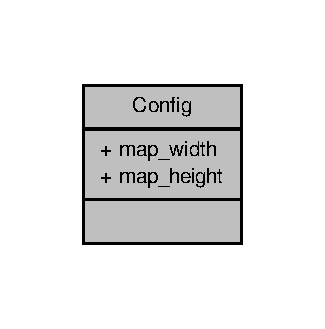
\includegraphics[width=156pt]{structConfig__coll__graph}
\end{center}
\end{figure}
\subsubsection*{Atrybuty publiczne}
\begin{DoxyCompactItemize}
\item 
\hypertarget{structConfig_ac4596f9cbfcf2ab612ef32c4a6fbb21d}{int {\bfseries map\-\_\-width}}\label{structConfig_ac4596f9cbfcf2ab612ef32c4a6fbb21d}

\item 
\hypertarget{structConfig_a2ab1bfe7f4004dfb2082204638493b55}{int {\bfseries map\-\_\-height}}\label{structConfig_a2ab1bfe7f4004dfb2082204638493b55}

\end{DoxyCompactItemize}


\subsubsection{Opis szczegółowy}
Klasa przechowujaca komplet ustawien wybranych przez uzytkownika na ekranie startowym. 

\begin{DoxyRefDesc}{Do zrobienia}
\item[\hyperlink{todo__todo000001}{Do zrobienia}]moze zrobmy z tego singleton? \end{DoxyRefDesc}


\subsubsection{Dokumentacja atrybutów składowych}
\hypertarget{structConfig_a2ab1bfe7f4004dfb2082204638493b55}{\index{Config@{Config}!map\-\_\-height@{map\-\_\-height}}
\index{map\-\_\-height@{map\-\_\-height}!Config@{Config}}
\paragraph[{map\-\_\-height}]{\setlength{\rightskip}{0pt plus 5cm}int Config\-::map\-\_\-height}}\label{structConfig_a2ab1bfe7f4004dfb2082204638493b55}
\hypertarget{structConfig_ac4596f9cbfcf2ab612ef32c4a6fbb21d}{\index{Config@{Config}!map\-\_\-width@{map\-\_\-width}}
\index{map\-\_\-width@{map\-\_\-width}!Config@{Config}}
\paragraph[{map\-\_\-width}]{\setlength{\rightskip}{0pt plus 5cm}int Config\-::map\-\_\-width}}\label{structConfig_ac4596f9cbfcf2ab612ef32c4a6fbb21d}


Dokumentacja dla tej struktury została wygenerowana z pliku\-:\begin{DoxyCompactItemize}
\item 
src/common/Config.\-hpp\end{DoxyCompactItemize}

\hypertarget{classCreature}{\subsection{Dokumentacja klasy Creature}
\label{classCreature}\index{Creature@{Creature}}
}


Abstrakcyjna klasa reprezentująca stworzenie.  




{\ttfamily \#include $<$Creature.\-hpp$>$}



Diagram dziedziczenia dla Creature
\nopagebreak
\begin{figure}[H]
\begin{center}
\leavevmode
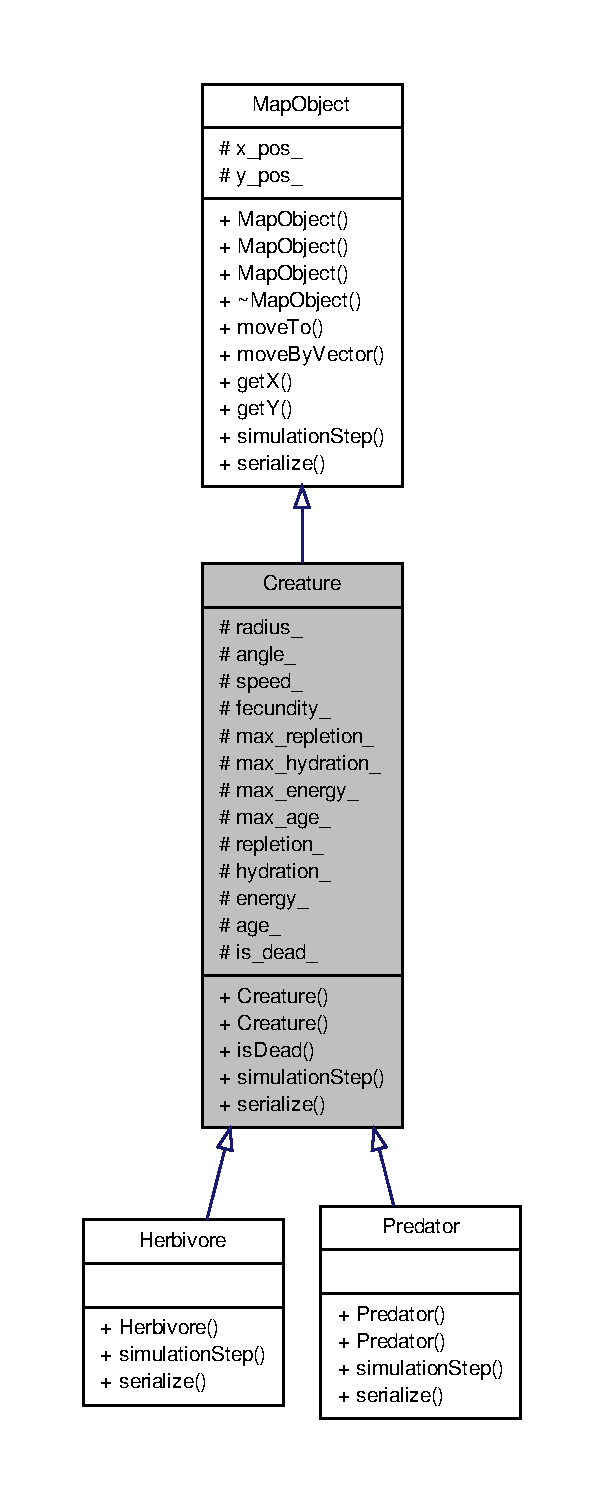
\includegraphics[height=550pt]{classCreature__inherit__graph}
\end{center}
\end{figure}


Diagram współpracy dla Creature\-:
\nopagebreak
\begin{figure}[H]
\begin{center}
\leavevmode
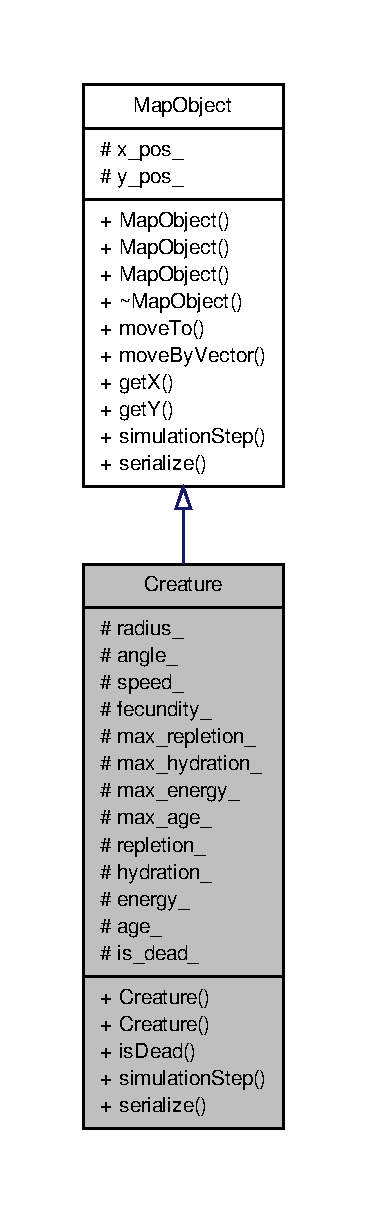
\includegraphics[height=550pt]{classCreature__coll__graph}
\end{center}
\end{figure}
\subsubsection*{Metody publiczne}
\begin{DoxyCompactItemize}
\item 
\hyperlink{classCreature_a85b135bb56773ebd20a30e7efc216a47}{Creature} (const \hyperlink{classCreature}{Creature} \&mother, const \hyperlink{classCreature}{Creature} \&father)
\begin{DoxyCompactList}\small\item\em Konstruktor wywoływany w momencie narodzin stworzenia. \end{DoxyCompactList}\item 
\hyperlink{classCreature_ab7aded4b4eee101b224e50985ca6d08d}{Creature} (double x\-\_\-pos, double y\-\_\-pos)
\begin{DoxyCompactList}\small\item\em Konstruktor wywoływany w przypadku, gdy stworzenie jest generowane na początku gry. \end{DoxyCompactList}\item 
bool \hyperlink{classCreature_ab4019c0b7940cd1b9fb19bf3399348ce}{is\-Dead} () const 
\begin{DoxyCompactList}\small\item\em Funkcja podaje informację czy stworzenie jest martwe. \end{DoxyCompactList}\item 
void \hyperlink{classCreature_af31d92f059f848284d371d3232384538}{simulation\-Step} (int miliseconds)=0
\begin{DoxyCompactList}\small\item\em Funkcja wykonuje jeden krok symulacji dla obiektu. \end{DoxyCompactList}\item 
{\footnotesize template$<$class Archive $>$ }\\void \hyperlink{classCreature_a03b0a51a8c6421046ce9ed004526566b}{serialize} (Archive \&ar, const unsigned int version)
\begin{DoxyCompactList}\small\item\em Serializacja. \end{DoxyCompactList}\end{DoxyCompactItemize}
\subsubsection*{Atrybuty chronione}
\begin{DoxyCompactItemize}
\item 
\hypertarget{classCreature_a319be828285119ac6d619bf1f926ada5}{const int \hyperlink{classCreature_a319be828285119ac6d619bf1f926ada5}{radius\-\_\-}}\label{classCreature_a319be828285119ac6d619bf1f926ada5}

\begin{DoxyCompactList}\small\item\em Zasięg widzenia. \end{DoxyCompactList}\item 
\hypertarget{classCreature_afa39083bf461c18b35a4c0deac5c68f1}{const int \hyperlink{classCreature_afa39083bf461c18b35a4c0deac5c68f1}{angle\-\_\-}}\label{classCreature_afa39083bf461c18b35a4c0deac5c68f1}

\begin{DoxyCompactList}\small\item\em Kąt widzenia. \end{DoxyCompactList}\item 
\hypertarget{classCreature_ae473a3d0259ba0da2516b8500009283a}{const int \hyperlink{classCreature_ae473a3d0259ba0da2516b8500009283a}{speed\-\_\-}}\label{classCreature_ae473a3d0259ba0da2516b8500009283a}

\begin{DoxyCompactList}\small\item\em Prędkość poruszania się \end{DoxyCompactList}\item 
\hypertarget{classCreature_a44c060eec028a0802ef4a0126139192b}{const int \hyperlink{classCreature_a44c060eec028a0802ef4a0126139192b}{fecundity\-\_\-}}\label{classCreature_a44c060eec028a0802ef4a0126139192b}

\begin{DoxyCompactList}\small\item\em Płodność \end{DoxyCompactList}\item 
\hypertarget{classCreature_ad7ac348b54af3efd118ef36b6c753962}{const int \hyperlink{classCreature_ad7ac348b54af3efd118ef36b6c753962}{max\-\_\-repletion\-\_\-}}\label{classCreature_ad7ac348b54af3efd118ef36b6c753962}

\begin{DoxyCompactList}\small\item\em Maksymalny poziom najedzenia (inaczej\-: odporność na głód) \end{DoxyCompactList}\item 
\hypertarget{classCreature_aaee7a3d9488cdeda758315440af15f30}{const int \hyperlink{classCreature_aaee7a3d9488cdeda758315440af15f30}{max\-\_\-hydration\-\_\-}}\label{classCreature_aaee7a3d9488cdeda758315440af15f30}

\begin{DoxyCompactList}\small\item\em Maksymalny poziom napojenia (inaczej\-: odporność na pragnienie) \end{DoxyCompactList}\item 
\hypertarget{classCreature_a30ca7a39a52b5dc36828fc2ea835a95f}{const int \hyperlink{classCreature_a30ca7a39a52b5dc36828fc2ea835a95f}{max\-\_\-energy\-\_\-}}\label{classCreature_a30ca7a39a52b5dc36828fc2ea835a95f}

\begin{DoxyCompactList}\small\item\em Maksymalny poziom energii (inaczej\-: odporność na zmęczenie) \end{DoxyCompactList}\item 
\hypertarget{classCreature_a3c85c0418b1036d292d4d598082626eb}{const int \hyperlink{classCreature_a3c85c0418b1036d292d4d598082626eb}{max\-\_\-age\-\_\-}}\label{classCreature_a3c85c0418b1036d292d4d598082626eb}

\begin{DoxyCompactList}\small\item\em Maksymalna długość życia. \end{DoxyCompactList}\item 
\hypertarget{classCreature_a48a77085b53f40477bfb6bfc2eb3f241}{double \hyperlink{classCreature_a48a77085b53f40477bfb6bfc2eb3f241}{repletion\-\_\-}}\label{classCreature_a48a77085b53f40477bfb6bfc2eb3f241}

\begin{DoxyCompactList}\small\item\em Obecny poziom najedzenia. \end{DoxyCompactList}\item 
\hypertarget{classCreature_a6650b16786f49d3dbc4dbde39ab21796}{double \hyperlink{classCreature_a6650b16786f49d3dbc4dbde39ab21796}{hydration\-\_\-}}\label{classCreature_a6650b16786f49d3dbc4dbde39ab21796}

\begin{DoxyCompactList}\small\item\em Obecny poziom napojenia. \end{DoxyCompactList}\item 
\hypertarget{classCreature_a64dae275114dc06c39eeb71d9f8e08ed}{double \hyperlink{classCreature_a64dae275114dc06c39eeb71d9f8e08ed}{energy\-\_\-}}\label{classCreature_a64dae275114dc06c39eeb71d9f8e08ed}

\begin{DoxyCompactList}\small\item\em Obecny poziom energii. \end{DoxyCompactList}\item 
\hypertarget{classCreature_abf62d53b9178d950e98fc0167f51b824}{double \hyperlink{classCreature_abf62d53b9178d950e98fc0167f51b824}{age\-\_\-}}\label{classCreature_abf62d53b9178d950e98fc0167f51b824}

\begin{DoxyCompactList}\small\item\em Obecny wiek. \end{DoxyCompactList}\item 
\hypertarget{classCreature_a55f70b769ee6a6be67a2ea23ac1b563f}{bool \hyperlink{classCreature_a55f70b769ee6a6be67a2ea23ac1b563f}{is\-\_\-dead\-\_\-}}\label{classCreature_a55f70b769ee6a6be67a2ea23ac1b563f}

\begin{DoxyCompactList}\small\item\em Czy zwierze jest martwe? \end{DoxyCompactList}\end{DoxyCompactItemize}


\subsubsection{Opis szczegółowy}
Abstrakcyjna klasa reprezentująca stworzenie. 

\subsubsection{Dokumentacja konstruktora i destruktora}
\hypertarget{classCreature_a85b135bb56773ebd20a30e7efc216a47}{\index{Creature@{Creature}!Creature@{Creature}}
\index{Creature@{Creature}!Creature@{Creature}}
\paragraph[{Creature}]{\setlength{\rightskip}{0pt plus 5cm}Creature\-::\-Creature (
\begin{DoxyParamCaption}
\item[{const {\bf Creature} \&}]{mother, }
\item[{const {\bf Creature} \&}]{father}
\end{DoxyParamCaption}
)\hspace{0.3cm}{\ttfamily [inline]}}}\label{classCreature_a85b135bb56773ebd20a30e7efc216a47}


Konstruktor wywoływany w momencie narodzin stworzenia. 

Parametry stworzenia są ustalane na podstawie odpowiednich parametrów ojca i matki.

Ten konstruktor zakłada, że matka i ojciec znajdują się w tym samym miejscu. Nowe stworzenie również pojawi się w tym samym miejscu.


\begin{DoxyParams}{Parametry}
{\em mother} & referencja do matki \\
\hline
{\em father} & referencja do ojca \\
\hline
\end{DoxyParams}
\begin{DoxyRefDesc}{Do zrobienia}
\item[\hyperlink{todo__todo000002}{Do zrobienia}]write me \end{DoxyRefDesc}
\hypertarget{classCreature_ab7aded4b4eee101b224e50985ca6d08d}{\index{Creature@{Creature}!Creature@{Creature}}
\index{Creature@{Creature}!Creature@{Creature}}
\paragraph[{Creature}]{\setlength{\rightskip}{0pt plus 5cm}Creature\-::\-Creature (
\begin{DoxyParamCaption}
\item[{double}]{x\-\_\-pos, }
\item[{double}]{y\-\_\-pos}
\end{DoxyParamCaption}
)\hspace{0.3cm}{\ttfamily [inline]}}}\label{classCreature_ab7aded4b4eee101b224e50985ca6d08d}


Konstruktor wywoływany w przypadku, gdy stworzenie jest generowane na początku gry. 

Wspolrzedne stworzenia są podawane jako parametry konstruktora.

Stworzenie pojawi się w wybranym miejscu na planszy (powinno ono byc wolne). \begin{DoxyRefDesc}{Do zrobienia}
\item[\hyperlink{todo__todo000003}{Do zrobienia}]write me \end{DoxyRefDesc}


\subsubsection{Dokumentacja funkcji składowych}
\hypertarget{classCreature_ab4019c0b7940cd1b9fb19bf3399348ce}{\index{Creature@{Creature}!is\-Dead@{is\-Dead}}
\index{is\-Dead@{is\-Dead}!Creature@{Creature}}
\paragraph[{is\-Dead}]{\setlength{\rightskip}{0pt plus 5cm}bool Creature\-::is\-Dead (
\begin{DoxyParamCaption}
{}
\end{DoxyParamCaption}
) const\hspace{0.3cm}{\ttfamily [inline]}}}\label{classCreature_ab4019c0b7940cd1b9fb19bf3399348ce}


Funkcja podaje informację czy stworzenie jest martwe. 

Dzieje się tak, gdy najedzenie, napojenie lub energia spadnie do zera lub gdy stworzenie osiągnie swój maksymalny wiek.

Po stwierdzeniu, że stworzenie jest martwe, funkcja nadrzędna powinna zniszczyć obiekt klasy \hyperlink{classCreature}{Creature}.

\begin{DoxyReturn}{Zwraca}
true wtedy i tylko wtedy gdy osobnik jest martwy. 
\end{DoxyReturn}
\begin{DoxyRefDesc}{Do zrobienia}
\item[\hyperlink{todo__todo000004}{Do zrobienia}]write me \end{DoxyRefDesc}
\hypertarget{classCreature_a03b0a51a8c6421046ce9ed004526566b}{\index{Creature@{Creature}!serialize@{serialize}}
\index{serialize@{serialize}!Creature@{Creature}}
\paragraph[{serialize}]{\setlength{\rightskip}{0pt plus 5cm}template$<$class Archive $>$ void Creature\-::serialize (
\begin{DoxyParamCaption}
\item[{Archive \&}]{ar, }
\item[{const unsigned int}]{version}
\end{DoxyParamCaption}
)\hspace{0.3cm}{\ttfamily [inline]}}}\label{classCreature_a03b0a51a8c6421046ce9ed004526566b}


Serializacja. 

Serializuje skladowe obiektu oraz klase bazowa.

\begin{DoxySeeAlso}{Zobacz również}
\hyperlink{classMap_a247075c0c8b390cdd3afab8f627d1e8d}{Map\-::serialize} 
\end{DoxySeeAlso}


Reimplementowana z \hyperlink{classMapObject_af7bd38411bbc26af1e0133538688d909}{Map\-Object}.



Reimplementowana w \hyperlink{classPredator_abf2e6236a7a0a26d97fbd6ebbfa09733}{Predator} i \hyperlink{classHerbivore_a05a43de5c6a5fa07fd3091692c3f4e94}{Herbivore}.

\hypertarget{classCreature_af31d92f059f848284d371d3232384538}{\index{Creature@{Creature}!simulation\-Step@{simulation\-Step}}
\index{simulation\-Step@{simulation\-Step}!Creature@{Creature}}
\paragraph[{simulation\-Step}]{\setlength{\rightskip}{0pt plus 5cm}void Creature\-::simulation\-Step (
\begin{DoxyParamCaption}
\item[{int}]{miliseconds}
\end{DoxyParamCaption}
)\hspace{0.3cm}{\ttfamily [pure virtual]}}}\label{classCreature_af31d92f059f848284d371d3232384538}


Funkcja wykonuje jeden krok symulacji dla obiektu. 


\begin{DoxyParams}{Parametry}
{\em miliseconds} & czas w milisekundach, który upłynął od poprzedniego kroku \\
\hline
\end{DoxyParams}


Implementuje \hyperlink{classMapObject_a8bd8926db59af00a61b8860352abfdd9}{Map\-Object}.



Implementowany w \hyperlink{classPredator_a7d8004ead868419138c8782fb392a1b1}{Predator} i \hyperlink{classHerbivore_a728f136b4489a168df89dadd244a86a8}{Herbivore}.



Dokumentacja dla tej klasy została wygenerowana z pliku\-:\begin{DoxyCompactItemize}
\item 
src/common/Creature.\-hpp\end{DoxyCompactItemize}

\hypertarget{classHerbivore}{\subsection{Dokumentacja klasy Herbivore}
\label{classHerbivore}\index{Herbivore@{Herbivore}}
}


Klasa reprezentujaca roslinozerce.  




{\ttfamily \#include $<$Herbivore.\-hpp$>$}



Diagram dziedziczenia dla Herbivore
\nopagebreak
\begin{figure}[H]
\begin{center}
\leavevmode
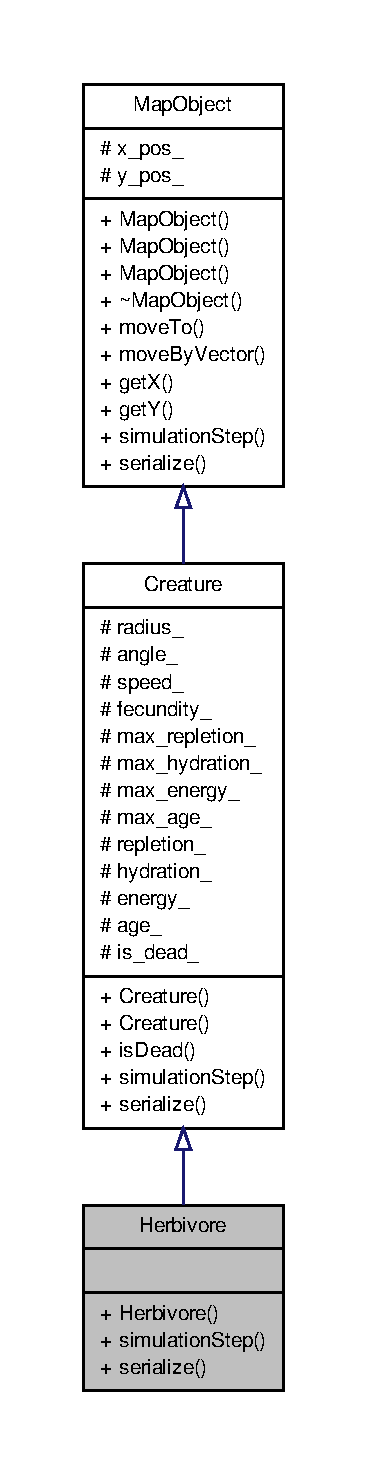
\includegraphics[height=550pt]{classHerbivore__inherit__graph}
\end{center}
\end{figure}


Diagram współpracy dla Herbivore\-:
\nopagebreak
\begin{figure}[H]
\begin{center}
\leavevmode
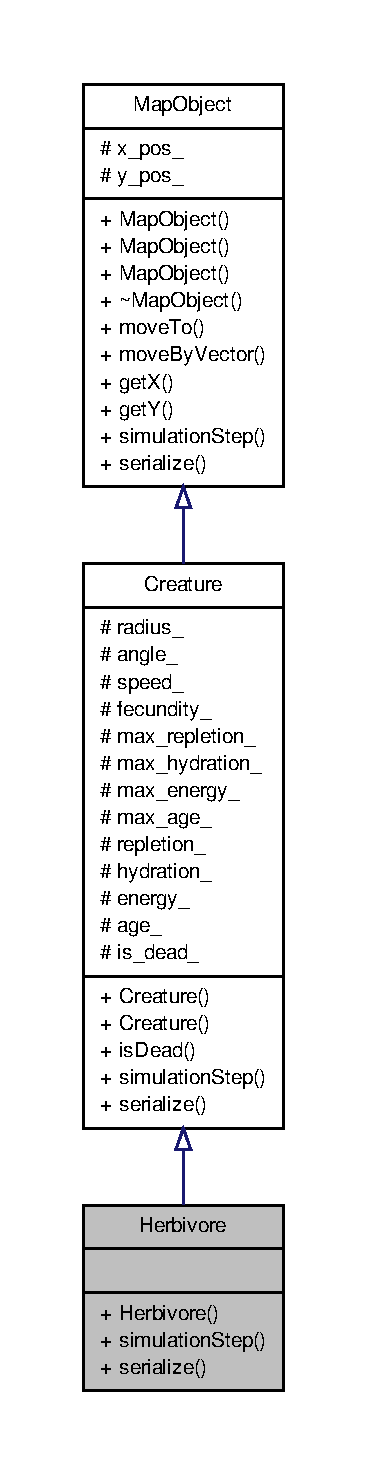
\includegraphics[height=550pt]{classHerbivore__coll__graph}
\end{center}
\end{figure}
\subsubsection*{Metody publiczne}
\begin{DoxyCompactItemize}
\item 
\hyperlink{classHerbivore_a2174349eed9903363d2840e0484a61d5}{Herbivore} (double x\-\_\-pos, double y\-\_\-pos)
\begin{DoxyCompactList}\small\item\em Konstruktor wywoływany w przypadku, gdy stworzenie jest generowane na początku gry. \end{DoxyCompactList}\item 
virtual void \hyperlink{classHerbivore_a728f136b4489a168df89dadd244a86a8}{simulation\-Step} (int miliseconds)
\begin{DoxyCompactList}\small\item\em Funkcja wykonuje jeden krok symulacji dla obiektu. \end{DoxyCompactList}\item 
{\footnotesize template$<$class Archive $>$ }\\void \hyperlink{classHerbivore_a05a43de5c6a5fa07fd3091692c3f4e94}{serialize} (Archive \&ar, const unsigned int version)
\begin{DoxyCompactList}\small\item\em Serializacja. \end{DoxyCompactList}\end{DoxyCompactItemize}
\subsubsection*{Dodatkowe Dziedziczone Składowe}


\subsubsection{Opis szczegółowy}
Klasa reprezentujaca roslinozerce. 

\begin{DoxyRefDesc}{Do zrobienia}
\item[\hyperlink{todo__todo000005}{Do zrobienia}]write me \end{DoxyRefDesc}


\subsubsection{Dokumentacja konstruktora i destruktora}
\hypertarget{classHerbivore_a2174349eed9903363d2840e0484a61d5}{\index{Herbivore@{Herbivore}!Herbivore@{Herbivore}}
\index{Herbivore@{Herbivore}!Herbivore@{Herbivore}}
\paragraph[{Herbivore}]{\setlength{\rightskip}{0pt plus 5cm}Herbivore\-::\-Herbivore (
\begin{DoxyParamCaption}
\item[{double}]{x\-\_\-pos, }
\item[{double}]{y\-\_\-pos}
\end{DoxyParamCaption}
)\hspace{0.3cm}{\ttfamily [inline]}}}\label{classHerbivore_a2174349eed9903363d2840e0484a61d5}


Konstruktor wywoływany w przypadku, gdy stworzenie jest generowane na początku gry. 

Wspolrzedne stworzenia są podawane jako parametry konstruktora.

Stworzenie pojawi się w wybranym miejscu na planszy (powinno ono byc wolne). 

\subsubsection{Dokumentacja funkcji składowych}
\hypertarget{classHerbivore_a05a43de5c6a5fa07fd3091692c3f4e94}{\index{Herbivore@{Herbivore}!serialize@{serialize}}
\index{serialize@{serialize}!Herbivore@{Herbivore}}
\paragraph[{serialize}]{\setlength{\rightskip}{0pt plus 5cm}template$<$class Archive $>$ void Herbivore\-::serialize (
\begin{DoxyParamCaption}
\item[{Archive \&}]{ar, }
\item[{const unsigned int}]{version}
\end{DoxyParamCaption}
)\hspace{0.3cm}{\ttfamily [inline]}}}\label{classHerbivore_a05a43de5c6a5fa07fd3091692c3f4e94}


Serializacja. 

\begin{DoxySeeAlso}{Zobacz również}
\hyperlink{classMap_a247075c0c8b390cdd3afab8f627d1e8d}{Map\-::serialize} 
\end{DoxySeeAlso}


Reimplementowana z \hyperlink{classCreature_a03b0a51a8c6421046ce9ed004526566b}{Creature}.

\hypertarget{classHerbivore_a728f136b4489a168df89dadd244a86a8}{\index{Herbivore@{Herbivore}!simulation\-Step@{simulation\-Step}}
\index{simulation\-Step@{simulation\-Step}!Herbivore@{Herbivore}}
\paragraph[{simulation\-Step}]{\setlength{\rightskip}{0pt plus 5cm}virtual void Herbivore\-::simulation\-Step (
\begin{DoxyParamCaption}
\item[{int}]{miliseconds}
\end{DoxyParamCaption}
)\hspace{0.3cm}{\ttfamily [inline]}, {\ttfamily [virtual]}}}\label{classHerbivore_a728f136b4489a168df89dadd244a86a8}


Funkcja wykonuje jeden krok symulacji dla obiektu. 

Poszczególne elementy symulacji (poszukiwanie pożywienia, poszukiwanie wody, polowanie, ucieczka, poszukiwanie schronienia, poszukiwanie partnera do reprodukcji) są wywoływane w odpowiedniej kolejności, wg piramidy potrzeb osobnika.


\begin{DoxyParams}{Parametry}
{\em miliseconds} & czas w milisekundach, który upłynął od poprzedniego kroku \\
\hline
\end{DoxyParams}


Implementuje \hyperlink{classCreature_af31d92f059f848284d371d3232384538}{Creature}.



Dokumentacja dla tej klasy została wygenerowana z pliku\-:\begin{DoxyCompactItemize}
\item 
src/common/Herbivore.\-hpp\end{DoxyCompactItemize}

\hypertarget{classMap}{\subsection{Dokumentacja klasy Map}
\label{classMap}\index{Map@{Map}}
}


Klasa reprezentujaca mape (obszar gry) wraz z zawartymi na niej obiektami.  




{\ttfamily \#include $<$Map.\-hpp$>$}



Diagram współpracy dla Map\-:
\nopagebreak
\begin{figure}[H]
\begin{center}
\leavevmode
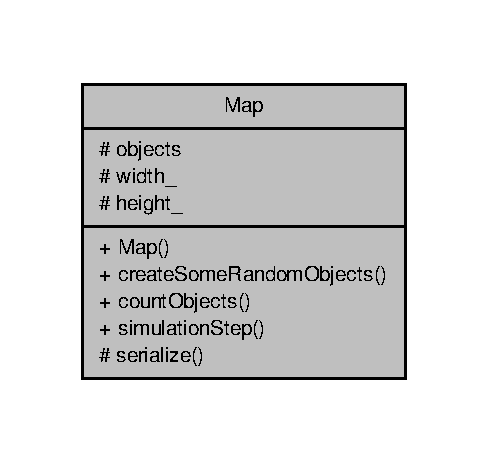
\includegraphics[width=234pt]{classMap__coll__graph}
\end{center}
\end{figure}
\subsubsection*{Metody publiczne}
\begin{DoxyCompactItemize}
\item 
\hypertarget{classMap_a8497952fd6e1f0584d868e6ceb97d42d}{\hyperlink{classMap_a8497952fd6e1f0584d868e6ceb97d42d}{Map} (int width, int height)}\label{classMap_a8497952fd6e1f0584d868e6ceb97d42d}

\begin{DoxyCompactList}\small\item\em Konstruktor tworzacy pusta mape o zadanych wymiarach. \end{DoxyCompactList}\item 
void \hyperlink{classMap_a2ea398c824a67d162ce4017b9173d685}{create\-Some\-Random\-Objects} ()
\begin{DoxyCompactList}\small\item\em T\-Y\-M\-C\-Z\-A\-S\-O\-W\-A F\-U\-N\-K\-C\-J\-A D\-O T\-E\-S\-T\-O\-W\-A\-N\-I\-A. \end{DoxyCompactList}\item 
int \hyperlink{classMap_ade3f961a8981ef66c159f968e4f98eb4}{count\-Objects} ()
\begin{DoxyCompactList}\small\item\em T\-Y\-M\-C\-Z\-A\-S\-O\-W\-A F\-U\-N\-K\-C\-J\-A D\-O T\-E\-S\-T\-O\-W\-A\-N\-I\-A. \end{DoxyCompactList}\item 
void \hyperlink{classMap_a71d87cb69a70ab3b3c2dc4ad39d13fcc}{simulation\-Step} (int miliseconds)
\begin{DoxyCompactList}\small\item\em Przeprowadza jeden krok symulacji dla wszystkich obiektow na mapie. \end{DoxyCompactList}\end{DoxyCompactItemize}
\subsubsection*{Metody chronione}
\begin{DoxyCompactItemize}
\item 
{\footnotesize template$<$class Archive $>$ }\\void \hyperlink{classMap_a247075c0c8b390cdd3afab8f627d1e8d}{serialize} (Archive \&ar, const unsigned int version)
\begin{DoxyCompactList}\small\item\em Serializacja (np na potrzeby zapisu/odczytu map na dysku) \end{DoxyCompactList}\end{DoxyCompactItemize}
\subsubsection*{Atrybuty chronione}
\begin{DoxyCompactItemize}
\item 
std\-::vector$<$ \hyperlink{classMapObject}{Map\-Object} $\ast$ $>$ \hyperlink{classMap_a77f2877faf3096da591f2e2d17d92a25}{objects}
\begin{DoxyCompactList}\small\item\em Wektor zawierający wszystkie obiekty znajdujące się na mapie. \end{DoxyCompactList}\item 
\hypertarget{classMap_a53b23c1478b2810098bddf1ba519e98f}{const int {\bfseries width\-\_\-}}\label{classMap_a53b23c1478b2810098bddf1ba519e98f}

\item 
\hypertarget{classMap_a0153ef0948d92b1761bf5ff8449e8337}{const int {\bfseries height\-\_\-}}\label{classMap_a0153ef0948d92b1761bf5ff8449e8337}

\end{DoxyCompactItemize}
\subsubsection*{Przyjaciele}
\begin{DoxyCompactItemize}
\item 
\hypertarget{classMap_ac98d07dd8f7b70e16ccb9a01abf56b9c}{class {\bfseries boost\-::serialization\-::access}}\label{classMap_ac98d07dd8f7b70e16ccb9a01abf56b9c}

\end{DoxyCompactItemize}


\subsubsection{Opis szczegółowy}
Klasa reprezentujaca mape (obszar gry) wraz z zawartymi na niej obiektami. 

Klasa może być serializowana przy pomocy boost\-::serialize

\begin{DoxyRefDesc}{Do zrobienia}
\item[\hyperlink{todo__todo000006}{Do zrobienia}]write me \end{DoxyRefDesc}


\subsubsection{Dokumentacja funkcji składowych}
\hypertarget{classMap_ade3f961a8981ef66c159f968e4f98eb4}{\index{Map@{Map}!count\-Objects@{count\-Objects}}
\index{count\-Objects@{count\-Objects}!Map@{Map}}
\paragraph[{count\-Objects}]{\setlength{\rightskip}{0pt plus 5cm}int Map\-::count\-Objects (
\begin{DoxyParamCaption}
{}
\end{DoxyParamCaption}
)\hspace{0.3cm}{\ttfamily [inline]}}}\label{classMap_ade3f961a8981ef66c159f968e4f98eb4}


T\-Y\-M\-C\-Z\-A\-S\-O\-W\-A F\-U\-N\-K\-C\-J\-A D\-O T\-E\-S\-T\-O\-W\-A\-N\-I\-A. 

\begin{DoxyRefDesc}{Do zrobienia}
\item[\hyperlink{todo__todo000008}{Do zrobienia}]U\-S\-U\-N M\-N\-I\-E G\-D\-Y N\-A\-P\-I\-S\-Z\-E\-S\-Z B\-A\-R\-D\-Z\-I\-E\-J Z\-A\-A\-W\-A\-N\-S\-O\-W\-A\-N\-E T\-E\-S\-T\-Y!!! \end{DoxyRefDesc}
\hypertarget{classMap_a2ea398c824a67d162ce4017b9173d685}{\index{Map@{Map}!create\-Some\-Random\-Objects@{create\-Some\-Random\-Objects}}
\index{create\-Some\-Random\-Objects@{create\-Some\-Random\-Objects}!Map@{Map}}
\paragraph[{create\-Some\-Random\-Objects}]{\setlength{\rightskip}{0pt plus 5cm}void Map\-::create\-Some\-Random\-Objects (
\begin{DoxyParamCaption}
{}
\end{DoxyParamCaption}
)\hspace{0.3cm}{\ttfamily [inline]}}}\label{classMap_a2ea398c824a67d162ce4017b9173d685}


T\-Y\-M\-C\-Z\-A\-S\-O\-W\-A F\-U\-N\-K\-C\-J\-A D\-O T\-E\-S\-T\-O\-W\-A\-N\-I\-A. 

\begin{DoxyRefDesc}{Do zrobienia}
\item[\hyperlink{todo__todo000007}{Do zrobienia}]U\-S\-U\-N M\-N\-I\-E G\-D\-Y N\-A\-P\-I\-S\-Z\-E\-S\-Z B\-A\-R\-D\-Z\-I\-E\-J Z\-A\-A\-W\-A\-N\-S\-O\-W\-A\-N\-E T\-E\-S\-T\-Y!!! \end{DoxyRefDesc}
\hypertarget{classMap_a247075c0c8b390cdd3afab8f627d1e8d}{\index{Map@{Map}!serialize@{serialize}}
\index{serialize@{serialize}!Map@{Map}}
\paragraph[{serialize}]{\setlength{\rightskip}{0pt plus 5cm}template$<$class Archive $>$ void Map\-::serialize (
\begin{DoxyParamCaption}
\item[{Archive \&}]{ar, }
\item[{const unsigned int}]{version}
\end{DoxyParamCaption}
)\hspace{0.3cm}{\ttfamily [inline]}, {\ttfamily [protected]}}}\label{classMap_a247075c0c8b390cdd3afab8f627d1e8d}


Serializacja (np na potrzeby zapisu/odczytu map na dysku) 

Do serializacji uzywamy boost\-::serialize. Aby prawidlowo serializowac klasy dziedziczace po \hyperlink{classMapObject}{Map\-Object}, nalezy uzyc makra B\-O\-O\-S\-T\-\_\-\-C\-L\-A\-S\-S\-\_\-\-E\-X\-P\-O\-R\-T w pliku cpp, w ktorym beda wolane metody serializacji.

Wiecej informacji\-: \href{http://stackoverflow.com/questions/3396330/where-to-put-boost-class-export-for-boostserialization}{\tt http\-://stackoverflow.\-com/questions/3396330/where-\/to-\/put-\/boost-\/class-\/export-\/for-\/boostserialization}

Obecnie metoda nie jest uzywana

\begin{DoxyRefDesc}{Do zrobienia}
\item[\hyperlink{todo__todo000010}{Do zrobienia}]uzyj mnie! \end{DoxyRefDesc}
\hypertarget{classMap_a71d87cb69a70ab3b3c2dc4ad39d13fcc}{\index{Map@{Map}!simulation\-Step@{simulation\-Step}}
\index{simulation\-Step@{simulation\-Step}!Map@{Map}}
\paragraph[{simulation\-Step}]{\setlength{\rightskip}{0pt plus 5cm}void Map\-::simulation\-Step (
\begin{DoxyParamCaption}
\item[{int}]{miliseconds}
\end{DoxyParamCaption}
)\hspace{0.3cm}{\ttfamily [inline]}}}\label{classMap_a71d87cb69a70ab3b3c2dc4ad39d13fcc}


Przeprowadza jeden krok symulacji dla wszystkich obiektow na mapie. 


\begin{DoxyParams}{Parametry}
{\em miliseconds} & czas w milisekundach, który upłynął od poprzedniego kroku \\
\hline
\end{DoxyParams}


\subsubsection{Dokumentacja atrybutów składowych}
\hypertarget{classMap_a77f2877faf3096da591f2e2d17d92a25}{\index{Map@{Map}!objects@{objects}}
\index{objects@{objects}!Map@{Map}}
\paragraph[{objects}]{\setlength{\rightskip}{0pt plus 5cm}std\-::vector$<${\bf Map\-Object} $\ast$$>$ Map\-::objects\hspace{0.3cm}{\ttfamily [protected]}}}\label{classMap_a77f2877faf3096da591f2e2d17d92a25}


Wektor zawierający wszystkie obiekty znajdujące się na mapie. 

Rozróżnienie typów obiektów zagwarantują wirtualne metody w hierarchii klas dziedziczących po typie \hyperlink{classMapObject}{Map\-Object}.

\begin{DoxyRefDesc}{Do zrobienia}
\item[\hyperlink{todo__todo000009}{Do zrobienia}]zmienic strukture danych na cos lepszego (moze mapa?) \end{DoxyRefDesc}


Dokumentacja dla tej klasy została wygenerowana z pliku\-:\begin{DoxyCompactItemize}
\item 
src/common/Map.\-hpp\end{DoxyCompactItemize}

\hypertarget{classMapObject}{\subsection{Dokumentacja klasy Map\-Object}
\label{classMapObject}\index{Map\-Object@{Map\-Object}}
}


Klasa abstrakcyjna reprezentująca dowolny obiekt znajdujący się na mapie (stworzenie, drzewo itp).  




{\ttfamily \#include $<$Map\-Object.\-hpp$>$}



Diagram dziedziczenia dla Map\-Object
\nopagebreak
\begin{figure}[H]
\begin{center}
\leavevmode
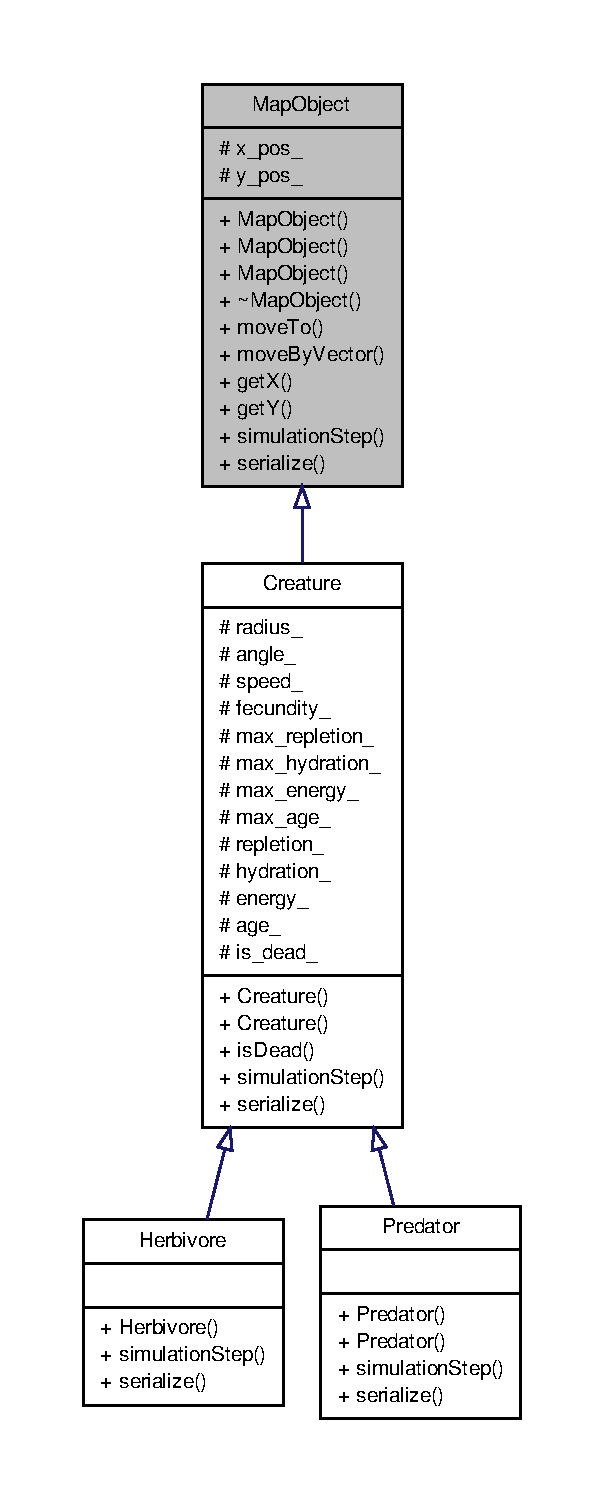
\includegraphics[height=550pt]{classMapObject__inherit__graph}
\end{center}
\end{figure}


Diagram współpracy dla Map\-Object\-:
\nopagebreak
\begin{figure}[H]
\begin{center}
\leavevmode
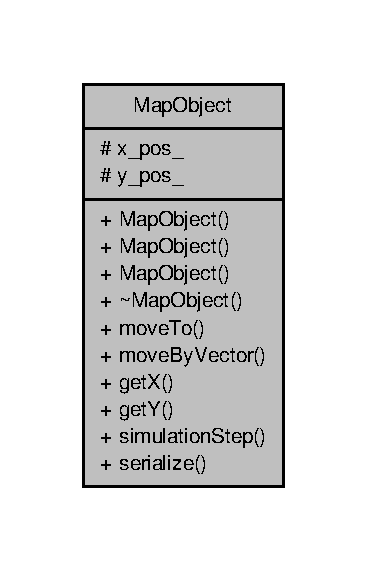
\includegraphics[width=176pt]{classMapObject__coll__graph}
\end{center}
\end{figure}
\subsubsection*{Metody publiczne}
\begin{DoxyCompactItemize}
\item 
\hypertarget{classMapObject_a568754515cc72ce0861d30c3040d26d2}{\hyperlink{classMapObject_a568754515cc72ce0861d30c3040d26d2}{Map\-Object} ()}\label{classMapObject_a568754515cc72ce0861d30c3040d26d2}

\begin{DoxyCompactList}\small\item\em konstruktor losujący pozycję dla obiektu \end{DoxyCompactList}\item 
\hypertarget{classMapObject_a2b742185ede789e5cb5beabb18e24eb2}{\hyperlink{classMapObject_a2b742185ede789e5cb5beabb18e24eb2}{Map\-Object} (double x\-\_\-pos, double y\-\_\-pos)}\label{classMapObject_a2b742185ede789e5cb5beabb18e24eb2}

\begin{DoxyCompactList}\small\item\em konstruktor z podaną pozycją startową \end{DoxyCompactList}\item 
\hypertarget{classMapObject_adbba6351e2a4a25fdd40d7c00ca37222}{\hyperlink{classMapObject_adbba6351e2a4a25fdd40d7c00ca37222}{Map\-Object} (const \hyperlink{classMapObject}{Map\-Object} \&another)}\label{classMapObject_adbba6351e2a4a25fdd40d7c00ca37222}

\begin{DoxyCompactList}\small\item\em konstruktor kopiujący pozycję z innego obiektu \end{DoxyCompactList}\item 
\hypertarget{classMapObject_a49b4b675ef2895fc05ef2eec72f4cd46}{void \hyperlink{classMapObject_a49b4b675ef2895fc05ef2eec72f4cd46}{move\-To} (double x\-\_\-pos, double y\-\_\-pos)}\label{classMapObject_a49b4b675ef2895fc05ef2eec72f4cd46}

\begin{DoxyCompactList}\small\item\em przemieszcza obiekt na zadaną pozycję \end{DoxyCompactList}\item 
\hypertarget{classMapObject_a9c111830e35093dd3b2f668c6d7d9736}{void \hyperlink{classMapObject_a9c111830e35093dd3b2f668c6d7d9736}{move\-By\-Vector} (double x\-\_\-vec, double y\-\_\-vec)}\label{classMapObject_a9c111830e35093dd3b2f668c6d7d9736}

\begin{DoxyCompactList}\small\item\em przemieszcza obiekt o zadany wektor \end{DoxyCompactList}\item 
\hypertarget{classMapObject_ad1a16784ebfef39db99b003b007e4aaa}{double \hyperlink{classMapObject_ad1a16784ebfef39db99b003b007e4aaa}{get\-X} () const }\label{classMapObject_ad1a16784ebfef39db99b003b007e4aaa}

\begin{DoxyCompactList}\small\item\em zwraca współrzędną X położenia \end{DoxyCompactList}\item 
\hypertarget{classMapObject_a1a14c2702a4afff02e8c037c1aebf73c}{double \hyperlink{classMapObject_a1a14c2702a4afff02e8c037c1aebf73c}{get\-Y} () const }\label{classMapObject_a1a14c2702a4afff02e8c037c1aebf73c}

\begin{DoxyCompactList}\small\item\em zwraca współrzędną Y położenia \end{DoxyCompactList}\item 
virtual void \hyperlink{classMapObject_a8bd8926db59af00a61b8860352abfdd9}{simulation\-Step} (int miliseconds)=0
\begin{DoxyCompactList}\small\item\em Funkcja wykonuje jeden krok symulacji dla obiektu. \end{DoxyCompactList}\item 
{\footnotesize template$<$class Archive $>$ }\\void \hyperlink{classMapObject_af7bd38411bbc26af1e0133538688d909}{serialize} (Archive \&ar, const unsigned int version)
\begin{DoxyCompactList}\small\item\em Serializacja. \end{DoxyCompactList}\end{DoxyCompactItemize}
\subsubsection*{Atrybuty chronione}
\begin{DoxyCompactItemize}
\item 
\hypertarget{classMapObject_a6083da4dfdf4efca1021a8486a40cd5f}{double \hyperlink{classMapObject_a6083da4dfdf4efca1021a8486a40cd5f}{x\-\_\-pos\-\_\-}}\label{classMapObject_a6083da4dfdf4efca1021a8486a40cd5f}

\begin{DoxyCompactList}\small\item\em składowa x położenia \end{DoxyCompactList}\item 
\hypertarget{classMapObject_afc248d9c7b5433767aa711d0a7a7399f}{double \hyperlink{classMapObject_afc248d9c7b5433767aa711d0a7a7399f}{y\-\_\-pos\-\_\-}}\label{classMapObject_afc248d9c7b5433767aa711d0a7a7399f}

\begin{DoxyCompactList}\small\item\em składowa y położenia \end{DoxyCompactList}\end{DoxyCompactItemize}


\subsubsection{Opis szczegółowy}
Klasa abstrakcyjna reprezentująca dowolny obiekt znajdujący się na mapie (stworzenie, drzewo itp). 

\subsubsection{Dokumentacja funkcji składowych}
\hypertarget{classMapObject_af7bd38411bbc26af1e0133538688d909}{\index{Map\-Object@{Map\-Object}!serialize@{serialize}}
\index{serialize@{serialize}!MapObject@{Map\-Object}}
\paragraph[{serialize}]{\setlength{\rightskip}{0pt plus 5cm}template$<$class Archive $>$ void Map\-Object\-::serialize (
\begin{DoxyParamCaption}
\item[{Archive \&}]{ar, }
\item[{const unsigned int}]{version}
\end{DoxyParamCaption}
)\hspace{0.3cm}{\ttfamily [inline]}}}\label{classMapObject_af7bd38411bbc26af1e0133538688d909}


Serializacja. 

\begin{DoxySeeAlso}{Zobacz również}
\hyperlink{classMap_a247075c0c8b390cdd3afab8f627d1e8d}{Map\-::serialize} 
\end{DoxySeeAlso}


Reimplementowana w \hyperlink{classCreature_a03b0a51a8c6421046ce9ed004526566b}{Creature}, \hyperlink{classPredator_abf2e6236a7a0a26d97fbd6ebbfa09733}{Predator} i \hyperlink{classHerbivore_a05a43de5c6a5fa07fd3091692c3f4e94}{Herbivore}.

\hypertarget{classMapObject_a8bd8926db59af00a61b8860352abfdd9}{\index{Map\-Object@{Map\-Object}!simulation\-Step@{simulation\-Step}}
\index{simulation\-Step@{simulation\-Step}!MapObject@{Map\-Object}}
\paragraph[{simulation\-Step}]{\setlength{\rightskip}{0pt plus 5cm}virtual void Map\-Object\-::simulation\-Step (
\begin{DoxyParamCaption}
\item[{int}]{miliseconds}
\end{DoxyParamCaption}
)\hspace{0.3cm}{\ttfamily [pure virtual]}}}\label{classMapObject_a8bd8926db59af00a61b8860352abfdd9}


Funkcja wykonuje jeden krok symulacji dla obiektu. 


\begin{DoxyParams}{Parametry}
{\em miliseconds} & czas w milisekundach, który upłynął od poprzedniego kroku \\
\hline
\end{DoxyParams}


Implementowany w \hyperlink{classCreature_af31d92f059f848284d371d3232384538}{Creature}, \hyperlink{classPredator_a7d8004ead868419138c8782fb392a1b1}{Predator} i \hyperlink{classHerbivore_a728f136b4489a168df89dadd244a86a8}{Herbivore}.



Dokumentacja dla tej klasy została wygenerowana z pliku\-:\begin{DoxyCompactItemize}
\item 
src/common/Map\-Object.\-hpp\end{DoxyCompactItemize}

\hypertarget{classPredator}{\subsection{Dokumentacja klasy Predator}
\label{classPredator}\index{Predator@{Predator}}
}


Klasa reprezentujaca drapieznika.  




{\ttfamily \#include $<$Predator.\-hpp$>$}



Diagram dziedziczenia dla Predator
\nopagebreak
\begin{figure}[H]
\begin{center}
\leavevmode
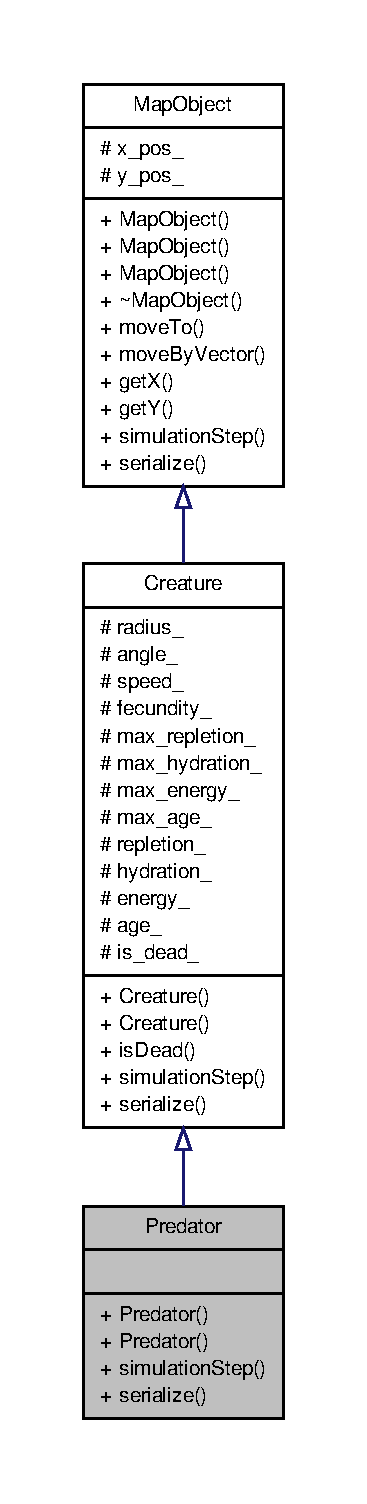
\includegraphics[height=550pt]{classPredator__inherit__graph}
\end{center}
\end{figure}


Diagram współpracy dla Predator\-:
\nopagebreak
\begin{figure}[H]
\begin{center}
\leavevmode
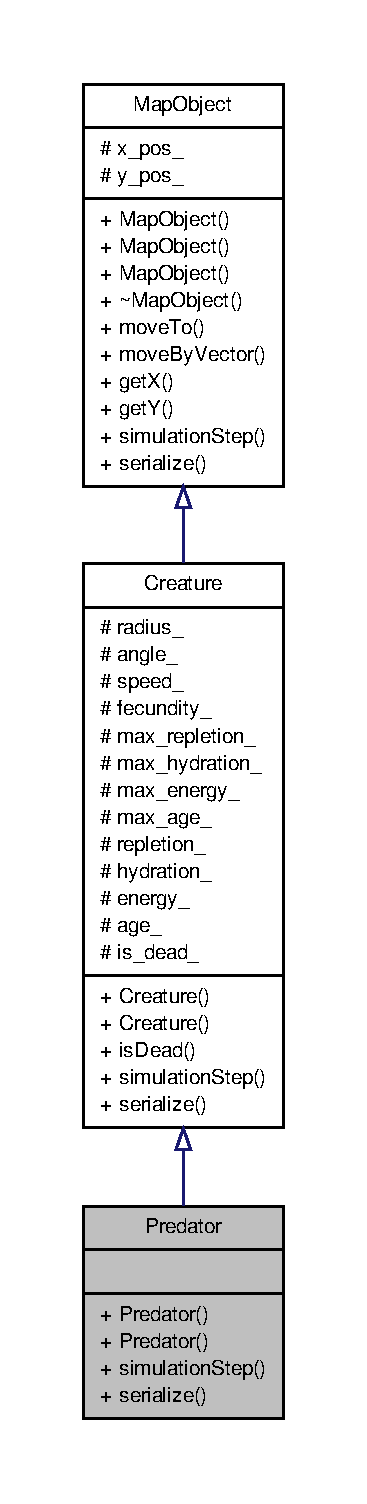
\includegraphics[height=550pt]{classPredator__coll__graph}
\end{center}
\end{figure}
\subsubsection*{Metody publiczne}
\begin{DoxyCompactItemize}
\item 
\hyperlink{classPredator_adebc1d4ae0858caf8ea906c167a32650}{Predator} (const \hyperlink{classPredator}{Predator} \&mother, const \hyperlink{classPredator}{Predator} \&father)
\begin{DoxyCompactList}\small\item\em Konstruktor wywoływany w momencie narodzin stworzenia. \end{DoxyCompactList}\item 
\hyperlink{classPredator_a889eb8b81088a0e9a0177c3f256e2413}{Predator} (double x\-\_\-pos, double y\-\_\-pos)
\begin{DoxyCompactList}\small\item\em Konstruktor wywoływany w przypadku, gdy stworzenie jest generowane na początku gry. \end{DoxyCompactList}\item 
virtual void \hyperlink{classPredator_a7d8004ead868419138c8782fb392a1b1}{simulation\-Step} (int miliseconds)
\begin{DoxyCompactList}\small\item\em Funkcja wykonuje jeden krok symulacji dla obiektu. \end{DoxyCompactList}\item 
{\footnotesize template$<$class Archive $>$ }\\void \hyperlink{classPredator_abf2e6236a7a0a26d97fbd6ebbfa09733}{serialize} (Archive \&ar, const unsigned int version)
\begin{DoxyCompactList}\small\item\em Serializacja. \end{DoxyCompactList}\end{DoxyCompactItemize}
\subsubsection*{Dodatkowe Dziedziczone Składowe}


\subsubsection{Opis szczegółowy}
Klasa reprezentujaca drapieznika. 

\subsubsection{Dokumentacja konstruktora i destruktora}
\hypertarget{classPredator_adebc1d4ae0858caf8ea906c167a32650}{\index{Predator@{Predator}!Predator@{Predator}}
\index{Predator@{Predator}!Predator@{Predator}}
\paragraph[{Predator}]{\setlength{\rightskip}{0pt plus 5cm}Predator\-::\-Predator (
\begin{DoxyParamCaption}
\item[{const {\bf Predator} \&}]{mother, }
\item[{const {\bf Predator} \&}]{father}
\end{DoxyParamCaption}
)\hspace{0.3cm}{\ttfamily [inline]}}}\label{classPredator_adebc1d4ae0858caf8ea906c167a32650}


Konstruktor wywoływany w momencie narodzin stworzenia. 

Parametry stworzenia są ustalane na podstawie odpowiednich parametrów ojca i matki.

Ten konstruktor zakłada, że matka i ojciec znajdują się w tym samym miejscu. Nowe stworzenie również pojawi się w tym samym miejscu.


\begin{DoxyParams}{Parametry}
{\em mother} & referencja do matki \\
\hline
{\em father} & referencja do ojca \\
\hline
\end{DoxyParams}
\hypertarget{classPredator_a889eb8b81088a0e9a0177c3f256e2413}{\index{Predator@{Predator}!Predator@{Predator}}
\index{Predator@{Predator}!Predator@{Predator}}
\paragraph[{Predator}]{\setlength{\rightskip}{0pt plus 5cm}Predator\-::\-Predator (
\begin{DoxyParamCaption}
\item[{double}]{x\-\_\-pos, }
\item[{double}]{y\-\_\-pos}
\end{DoxyParamCaption}
)\hspace{0.3cm}{\ttfamily [inline]}}}\label{classPredator_a889eb8b81088a0e9a0177c3f256e2413}


Konstruktor wywoływany w przypadku, gdy stworzenie jest generowane na początku gry. 

Wspolrzedne stworzenia są podawane jako parametry konstruktora.

Stworzenie pojawi się w wybranym miejscu na planszy (powinno ono byc wolne). 

\subsubsection{Dokumentacja funkcji składowych}
\hypertarget{classPredator_abf2e6236a7a0a26d97fbd6ebbfa09733}{\index{Predator@{Predator}!serialize@{serialize}}
\index{serialize@{serialize}!Predator@{Predator}}
\paragraph[{serialize}]{\setlength{\rightskip}{0pt plus 5cm}template$<$class Archive $>$ void Predator\-::serialize (
\begin{DoxyParamCaption}
\item[{Archive \&}]{ar, }
\item[{const unsigned int}]{version}
\end{DoxyParamCaption}
)\hspace{0.3cm}{\ttfamily [inline]}}}\label{classPredator_abf2e6236a7a0a26d97fbd6ebbfa09733}


Serializacja. 

\begin{DoxySeeAlso}{Zobacz również}
\hyperlink{classMap_a247075c0c8b390cdd3afab8f627d1e8d}{Map\-::serialize} 
\end{DoxySeeAlso}


Reimplementowana z \hyperlink{classCreature_a03b0a51a8c6421046ce9ed004526566b}{Creature}.

\hypertarget{classPredator_a7d8004ead868419138c8782fb392a1b1}{\index{Predator@{Predator}!simulation\-Step@{simulation\-Step}}
\index{simulation\-Step@{simulation\-Step}!Predator@{Predator}}
\paragraph[{simulation\-Step}]{\setlength{\rightskip}{0pt plus 5cm}virtual void Predator\-::simulation\-Step (
\begin{DoxyParamCaption}
\item[{int}]{miliseconds}
\end{DoxyParamCaption}
)\hspace{0.3cm}{\ttfamily [inline]}, {\ttfamily [virtual]}}}\label{classPredator_a7d8004ead868419138c8782fb392a1b1}


Funkcja wykonuje jeden krok symulacji dla obiektu. 

Poszczególne elementy symulacji (poszukiwanie pożywienia, poszukiwanie wody, polowanie, ucieczka, poszukiwanie schronienia, poszukiwanie partnera do reprodukcji) są wywoływane w odpowiedniej kolejności, wg piramidy potrzeb osobnika.


\begin{DoxyParams}{Parametry}
{\em miliseconds} & czas w milisekundach, który upłynął od poprzedniego kroku \\
\hline
\end{DoxyParams}


Implementuje \hyperlink{classCreature_af31d92f059f848284d371d3232384538}{Creature}.



Dokumentacja dla tej klasy została wygenerowana z pliku\-:\begin{DoxyCompactItemize}
\item 
src/common/Predator.\-hpp\end{DoxyCompactItemize}

\printindex
\end{document}
